\section{Marco Teórico}
\graphicspath{ {./intro/} }

\begin{frame}{Simulación de Modelos Matemáticos}
\frametitle{Modelos Matemáticos}

% \begin{block}{Definición de Modelo Matemático}
% Construcción matemática abstracta y simplificada relacionada con una parte
% de la realidad y creada para un propósito particular.
% \end{block}

\begin{block}{Definición de Modelo Matemático}
Conjunto de expresiones matemáticas (ecuaciones, inecuaciones,
ecuaciones diferenciales) que representan un sistema.
\end{block}

\begin{block}{Simulación}
    La simulación de un modelo consiste en la ejecución del
    mismo a través del tiempo.
\end{block}

\vspace{1em}

\centering
\pause

\textbf{Problema: Modelos complejos acarrean alto costo computacional}

\pause

\vspace{1em}

\textbf{Solución: Simulación en Paralelo}

\end{frame}


% \begin{frame}{Simulación de Modelos Matemáticos}
% \frametitle{Simulación de Modelos Matemáticos}

% Los modelos pueden clasificarse según la forma en que las variables
% evolucionan en el tiempo:

% \begin{itemize}
%     \item Modelos de Tiempo Discreto

%     \item Modelos de Tiempo Continuo
%     %acá puedo saltar a otra presentación y mostrar el ejemplo de discontinuidad?

%     \item Modelos de Eventos Discretos

%     \begin{itemize}
%         \item Método de los Sistemas de Estados Cuantificados (QSS)
%     \end{itemize}
% \end{itemize}

% \pause

% \centering

% \vspace{1em}

% \textbf{Problema: Modelos complejos acarrean alto costo computacional}

% \pause

% \vspace{1em}

% \textbf{Solución: Simulación en Paralelo}

% \end{frame}


% \begin{frame}{Simulación en Paralelo}

% Enfoques para la simulación en paralelo:

% \begin{itemize}
% \item \textbf{Algoritmos conservadores:}
%     \begin{itemize}
%         \item Fuerza a cada submodelo a esperar. Se asegura que no recibirá mensajes pasados.
%         \item Pequeñas mejoras de tiempo. Posibles bloqueos mutuos.
%     \end{itemize}
% \item \textbf{Algoritmos optimistas:}
%     \begin{itemize}
%         \item Avanza tanto como puede. Retrocede si hay una inconsistencia.
%         \item Más paralelismo. Guarda estructuras internas y el retroceso es costoso.
%     \end{itemize}
% \item \textbf{Algoritmos totalmente desincronizados:}
%     \begin{itemize}
%         \item Evita la sincronización por completo.
%         \item Grandes mejoras de tiempo. Introduce errores.
%     \end{itemize}
% \end{itemize}

% \end{frame}

% \begin{frame}{Simulación en Paralelo}

% Idea general:\pause

% \vspace{1em}

% Particionar el modelo entre \textbf{P submodelos}, donde cada submodelo se simula en un hilo 
% de ejecución diferente.\pause

% En cada paso de simulación, cada submodelo chequa si la variable que cambió se debe informar a los demás.\pause

% % Por ejemplo: para modelos QSS se usa sincronización no estricta, se calcula un tiempo virtual global y ningún submodelo
% % avanza más allá de ese tiempo mínimo y un valor proveído por el usuario.

% \end{frame}


\begin{frame}{Simulación en Paralelo}

Los algoritmos de simulación en paralelo requieren que:


\begin{itemize}
    \item El modelo original sea divido en $P$ submodelos.

    \item Cada submodelo sea simulado por un hilo diferente.

\end{itemize}

\pause

Para obtener una paralelización efectiva:

\begin{itemize}
    \item La \textbf{partición} del modelo debe ser \textbf{balanceada}.

    \item La \textbf{comunicación} entre los submodelos debe ser \textbf{minimizada}.

\end{itemize}

\pause
Requieren que \textbf{particionemos el modelo}. \pause
Llamamos a este proceso \textit{Balance de carga}.

\end{frame}


\begin{frame}{Balance de Carga para Simulación en Paralelo}

Podemos distinguir tres tipos de problemas de balance de carga:

\only<1>{
\begin{itemize}
    \item \textbf{Balance de carga estático}: la asignación a los procesadores se realiza al inicio de la simulación. % sin tener ninguna informacion sobre los resultados reales de la simulación.
    \item \textbf{Balance de carga semi-estático}: la asignación a los procesadores
ocurre al comienzo de la simulación, pero una conocimiento de dominio
extra. %u otra información relacionada puede ser aprovechada para mejorar
%la solución lacanzada.
    \item \textbf{Balance de carga dinámico}: la asignación a los procesadores se hace
dinámicamente en el transcurso de la simulación.
\end{itemize}
\vspace{2em}
}

\only<2>{
\begin{itemize}
    \item {\textbf{Balance de carga estático}}: la asignación a los procesadores se realiza al 
    inicio de la simulación. % sin tener ninguna informacion sobre los resultados reales de 
    % la simulación.
    \item {\color{gray}{Balance de carga semi-estático}: la asignación a los 
    procesadores ocurre al comienzo de la simulación, pero una conocimiento de dominio
extra.} %u otra información relacionada puede ser aprovechada para mejorar
%la solución lacanzada.
    \item {\color{gray}{Balance de carga dinámico}: la asignación a los procesadores se 
    hace dinámicamente en el transcurso de la simulación.}
\end{itemize}
\vspace{2em}
}

\only<3->{
\begin{itemize}
    \item {\textbf{Balance de carga estático}}: la asignación a los procesadores se realiza al 
    inicio de la simulación. % sin tener ninguna informacion sobre los resultados reales de 
    % la simulación.
    \item {\color{gray}{Balance de carga semi-estático}: la asignación a los 
    procesadores ocurre al comienzo de la simulación, pero una conocimiento de dominio
extra.} %u otra información relacionada puede ser aprovechada para mejorar
%la solución lacanzada.
    \item {\color{gray}{Balance de carga dinámico}: la asignación a los procesadores se 
    hace dinámicamente en el transcurso de la simulación.}
\end{itemize}
\pause
El problema de balance de carga se puede tratarse como un problema de
\textbf{particionamiento de grafos}.
}

\end{frame}


\begin{frame}{Métodos de Particionamiento de Grafos}

\begin{itemize}
    \item \textbf{Métodos geométricos.}

    \begin{itemize}
        \footnotesize
        \item Agrupan por coordenadas geométricas.

        \item Son rápidos y fáciles de implementar.

        \item Inducen costos altos de comunicación.
    \end{itemize}

    \item \textbf{Métodos combinatorios.}

    \begin{itemize}
        \footnotesize
        \item Agrupan según la adyacencia del grafo.

        \item Particiones de mejor calidad.

        \item Más demandantes computacionalmente.

    \end{itemize}

    \item \textbf{Métodos espectrales.}
    \begin{itemize}
        \footnotesize
        \item Calculan una distancia basada en conectividad y dividen balanceadamente.

        \item Produce particionamientos de alta calidad.

        \item Escalan ineficientemente cuando el tamaño del grafo crece.
    \end{itemize}

    \item \textbf{Métodos multinivel.}

    \begin{itemize}
        \footnotesize
        \item Arma el grafo, compacta, refina y expande el grafo.

        \item Son lo más utilizados en esta área. Producen particiones de alta calidad.

        \item La compactación y expansión del grafo es más costosa cuando el grafo crece.
    \end{itemize}
\end{itemize}
\pause
\centering
\textbf{¿Cómo construímos dicho grafo?}

\end{frame}


\begin{frame}{Grafo Computacional}


Las unidades de cálculo y sus dependencias se pueden modelar de forma natural
mediante un \textbf{grafo no dirigido}.

Más especificamente, $\mathcal{G} = (\mathcal{V}, \mathcal{E}, l, 
w)$, donde:

\vspace{1em}

$\mathcal{V} \hspace{2em} \text{el conjunto de nodos/las unidades de computación más pequeñas}$

$\mathcal{E}: \mathcal{E} \subset \mathcal{V} \times \mathcal{V} 
\hspace{2em} \text{el conjunto de aristas/dependencias entre unidades}$

$l: \mathcal{V} \to \mathcal{R}^+ \hspace{2em} 
\text{asigna un peso computacional a cada nodo}$

$w: \mathcal{E} \to \mathcal{R}^+ \hspace{2em} 
\text{asigna un peso comunicacional a cada arista} $

\vspace {1em}

Este grafo se conoce como \textbf{Grafo Computacional}.

\pause

\vspace {1em}

Necesitamos una forma de obtener dicho grafo computacional $\mathcal{G}$
de un modelo implementado en \textbf{Modelica}.

\end{frame}


\begin{frame}[fragile]{Modelo Advección-Difusión-Reacción}

Lo siguiente es un fragmento de una implementación en Modelica de un modelo
Advección-Difusión-Reacción (ADR):

  \begin{center}
    \begin{tabular}{c}
    \lstset{
        basicstyle=\scriptsize,
        emph={u},
        emphstyle=\color{red},
        morekeywords={u},
        keywordstyle=\bfseries,
        escapeinside={(*@}{@*)}
    }
      \begin{lstlisting}
          Real u[N];
          ...
          der(u[1])=-a*(u[1]-1)/dx+d*(-2*u[1]+1)/(dx^2)+r*(u[1]^2)*(1-u[1]);
          for i in 2:N loop
            der(u[i])=-a*(u[i]-u[i-1])/dx+ d*(-2*u[i]+u[i-1])/(dx^2)+ 
            r*(u[i]^2)*(1-u[i]);
          end for;
      \end{lstlisting}
    \end{tabular}
  \end{center}

  Queremos poder construir su grafo computacional a partir de su implementación.

  \pause

  Ejemplo para $N=10$.

  \footnotesize
  \begin{center}
        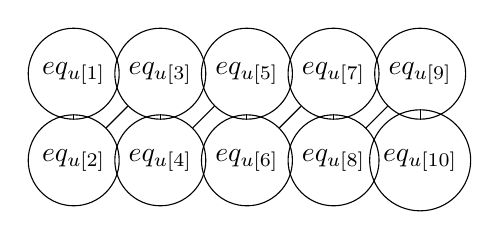
\begin{tikzpicture}[main/.style = {draw, circle}] 
            \node[main] (1) {$eq_{u[1]}$};
            \node[main] (2) [below of=1, node distance=11mm] {$eq_{u[2]}$}; 
            \node[main] (3) [right of=1, node distance=11mm] {$eq_{u[3]}$};
            \node[main] (4) [below of=3, node distance=11mm] {$eq_{u[4]}$};
            \node[main] (5) [right of=3, node distance=11mm] {$eq_{u[5]}$};
            \node[main] (6) [below of=5, node distance=11mm] {$eq_{u[6]}$}; 
            \node[main] (7) [right of=5, node distance=11mm] {$eq_{u[7]}$};
            \node[main] (8) [below of=7, node distance=11mm] {$eq_{u[8]}$}; 
            \node[main] (9) [right of=7, node distance=11mm] {$eq_{u[9]}$};
            \node[main] (10) [below of=9, node distance=11mm] {$eq_{u[10]}$};
        \pause
            \draw (1) -- (2);
        \pause
            \draw (2) -- (3);
        \pause
            \draw (3) -- (4);
            \draw (4) -- (5);
            \draw (5) -- (6);
            \draw (6) -- (7);
            \draw (7) -- (8);
            \draw (8) -- (9);
            \draw (9) -- (10);
    
        \end{tikzpicture}       
  \end{center}

\end{frame}


\begin{frame}{Mejoras en el Balance de Carga}

    Los algoritmos \textbf{multinivel} crean el graho, compactan, mejoran las
    particiones iniciales y expanden el grafo nuevamente.

    Queremos evitar dicha compactación y posterior expansión,
    buscamos aprovechar la naturaleza cíclica de \textbf{Modelica}.

    Veamos una estructura de datos que nos permite representar grafos en forma compacta.

\end{frame}


\begin{frame}{Grafos Basados en Conjuntos}

Un Grafo Basado en Conjuntos (SBG) no dirigido es una tupla
$\mathcal{G} = (\mathcal{V}, \mathcal{E}, map_1, map_2)$ donde:

\begin{itemize}
    \item $\mathcal{V} = \{V_1, \ldots, V_n \}$ es un conjunto de 
    vértices-conjunto disjuntos.

    \item $\mathcal{E} = \{E_1, \ldots, E_m \}$ es un conjunto de 
    aristas-conjunto que une vértices-conjunto de $\mathcal{V}$.

    \item $map_1 : \mathcal{E} \to \mathcal{V}$ tal que dado
    $e \in \mathcal{E}$, $map_1(e)$ representa uno de los extremos
    de la arista $e$.

    \item $map_2 : \mathcal{E} \to \mathcal{V}$ tal que dado
    $e \in \mathcal{E}$, $map_2(e)$ representa el otro de los
    extremos de la arista $e$.
\end{itemize}

\end{frame}

\begin{frame}{Grafos Basados en Conjuntos}

Sea $G = (V,E)$ un grafo tradicional no dirigido donde:

\scriptsize
\begin{itemize}
    \item \scriptsize $V = \{1, \ldots, 10\}$ \small son sus vértices-conjunto.
    \item \scriptsize $E = \{ \{1,2\}, \{2,3\}, \{3,4\}, \{4,5\}, \{5,6\}, 
    \{6,7\}, \{7,8\}, \{8,9\},\{9,10\} \}$ \small son sus aristas-conjunto.
\end{itemize}


\small
Una definición equivalente del mismo usando un SBG

$\mathcal{G} = (\mathcal{V}, \mathcal{E}, map_1, map_2)$ donde:

\begin{itemize}
    \item \scriptsize $\mathcal{V} = \{[1:1], [2:10]\}$ \small son sus nodos.
    \item \scriptsize $\mathcal{E} = \{ [1:1], [2:9] \}$ \small son sus aristas.
    \item Y sus mapas pueden defirse por medio de funciones por partes \scriptsize
    \[
        map_1(e)= \left \{ \begin {array} {ll}
                           1 & \text{si } e \in [1:1] \\
                           e + 1 & \text{si } e \in [2:9] \\
                         \end {array} \right.
    \]

    \[
        map_2(e)= \left \{ \begin {array} {ll}
                           e + 1 & \text{si } e \in [1:1] \\
                           e & \text{si } e \in [2:9] \\
                         \end {array} \right.
    \]

\end{itemize}

\end{frame}

\begin{frame}{Grafos Basados en Conjuntos}

En la descripción gráfico del grafo $G$, o su equivalente $\mathcal{G}$, definido
previamente:

\begin{itemize}
    \item las  aristas correspondientes al intervalo $[1:1]$ están en color rojo.
    \item las correspondientes al intervalo $[2:9]$ en negro.
\end{itemize}

\vspace{1em}

\centering

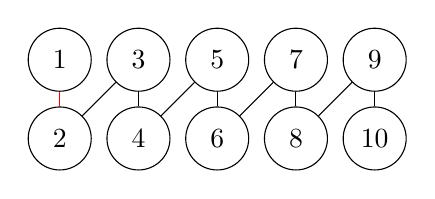
\begin{tikzpicture}[main/.style = {draw, circle}] 
    \node[main] (1) [minimum height=8mm] {$1$};
    \node[main] (2) [minimum height=8mm,below of=1, node distance=10mm] {$2$}; 
    \node[main] (3) [minimum height=8mm,right of=1, node distance=10mm] {$3$};
    \node[main] (4) [minimum height=8mm,below of=3, node distance=10mm] {$4$};
    \node[main] (5) [minimum height=8mm,right of=3, node distance=10mm] {$5$};
    \node[main] (6) [minimum height=8mm,below of=5, node distance=10mm] {$6$}; 
    \node[main] (7) [minimum height=8mm,right of=5, node distance=10mm] {$7$};
    \node[main] (8) [minimum height=8mm,below of=7, node distance=10mm] {$8$}; 
    \node[main] (9) [minimum height=8mm, right of=7, node distance=10mm] {$9$};
    \node[main] (10) [minimum height=8mm,below of=9, node distance=10mm] {$10$};

    \draw (1) -- (2) [color=red];
    \draw (2) -- (3);
    \draw (3) -- (4);
    \draw (4) -- (5);
    \draw (5) -- (6);
    \draw (6) -- (7);
    \draw (7) -- (8);
    \draw (8) -- (9);
    \draw (9) -- (10);

\end{tikzpicture}

\footnotesize
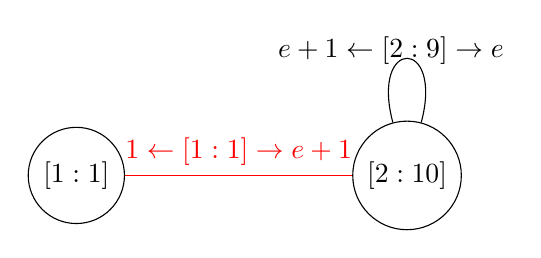
\begin{tikzpicture}[main/.style = {draw, circle}] 

    \node[main] (1) {$[1:1]$};
    \node[main] (2) [right of=1, node distance=42mm] {$[2:10]$};

    \draw[color=red] (1) -- (2) node [midway, above] {$1 \gets [1:1] \to e + 1$};
    \draw[loop above, color=black] (2) to node[near start, above] {$e + 1 \gets [2:9] \to e$} (2);

\end{tikzpicture}

\end{frame}


\begin{frame}{Grafos Basados en Conjuntos y Modelica}
    \centering
    
\includegraphics[width=0.5\textwidth]{simpsons.jpg}

    ¿Cómo podríamos construir un grafo computacional basado en conjuntos
    a partir de un modelo implementado en Modelica?
\end{frame}